\let\negmedspace\undefined
\let\negthickspace\undefined
\documentclass[journal]{IEEEtran}
\usepackage[a5paper, margin=10mm, onecolumn]{geometry}
%\usepackage{lmodern} % Ensure lmodern is loaded for pdflatex
\usepackage{tfrupee} % Include tfrupee package

\setlength{\headheight}{1cm} % Set the height of the header box
\setlength{\headsep}{0mm}     % Set the distance between the header box and the top of the text

\usepackage{gvv-book}
\usepackage{gvv}
\usepackage{cite}
\usepackage{amsmath,amssymb,amsfonts,amsthm}
\usepackage{algorithmic}
\usepackage{graphicx}
\usepackage{textcomp}
\usepackage{xcolor}
\usepackage{txfonts}
\usepackage{listings}
\usepackage{enumitem}
\usepackage{mathtools}
\usepackage{gensymb}
\usepackage{comment}
\usepackage[breaklinks=true]{hyperref}
\usepackage{tkz-euclide} 
\usepackage{listings}
% \usepackage{gvv}                                        
\def\inputGnumericTable{}                                 
\usepackage[latin1]{inputenc}                                
\usepackage{color}                                            
\usepackage{array}                                            
\usepackage{longtable}                                       
\usepackage{calc}                                             
\usepackage{multirow}                                         
\usepackage{hhline}                                           
\usepackage{ifthen}                                           
\usepackage{lscape}
\begin{document}
	
	\bibliographystyle{IEEEtran}
	\vspace{3cm}
	
	\title{4.4.2.22}
	\author{EE24BTECH11059 - Yellanki Siddhanth
	}
	% \maketitle
	% \newpage
	% \bigskip
	{\let\newpage\relax\maketitle}
	
	\renewcommand{\thefigure}{\theenumi}
	\renewcommand{\thetable}{\theenumi}
	\setlength{\intextsep}{10pt} % Space between text and floats
	
	
	\numberwithin{equation}{enumi}
	\numberwithin{figure}{enumi}
	\renewcommand{\thetable}{\theenumi}
	
\textbf{Question: }\\
Show that two lines  $a_1 x+ b_1y + c_1 = 0 $and $a_2 x+ b_2 y + c_2 = 0$ where $b_1 b_2 \neq 0$ are parallel if
$\frac{a_1}{b_1} = \frac{a_2}{b_2}$
\textbf{Solution: } \\
\begin{table}[h!]    
	\centering
	

	\caption{}
\end{table}\\
Rewriting both the lines in $n^\top x = c$ form,
	\begin{align}
		L_1 \equiv n_1^\top x = -c_1
	\end{align}
	\begin{align}
		n_1 = \myvec{a_1 \\ b_1}  \implies 		\norm{n_1} = \sqrt{a_1^2 + b_1^2}
	\end{align}
	\begin{align}
		L_2 \equiv n_2^\top x = -c_2
	\end{align}
	\begin{align}
		n_2 = \myvec{a_2 \\ b_2}  \implies 		\norm{n_2} = \sqrt{a_2^2 + b_2^2}
	\end{align}
If $L_1$ and $L_2$ are parallel lines, then their direction cosines must be the same.
	\begin{align}
		\frac{n_2}{\norm{n_2}} = \frac{n_1}{\norm{n_1}}\\
		 \implies \frac{a_1}{\sqrt{a_1^2 + b_1^2}} = \frac{a_2}{\sqrt{a_2^2 + b_2^2}}\\
		 \implies \frac{b_1}{\sqrt{a_1^2 + b_1^2}} = \frac{b_2}{\sqrt{a_2^2 + b_2^2}}
	\end{align}
	Thus proving that $\frac{a_1}{b_1} = \frac{a_2}{b_2}$.\\
	\begin{figure}[h!]
		\centering
		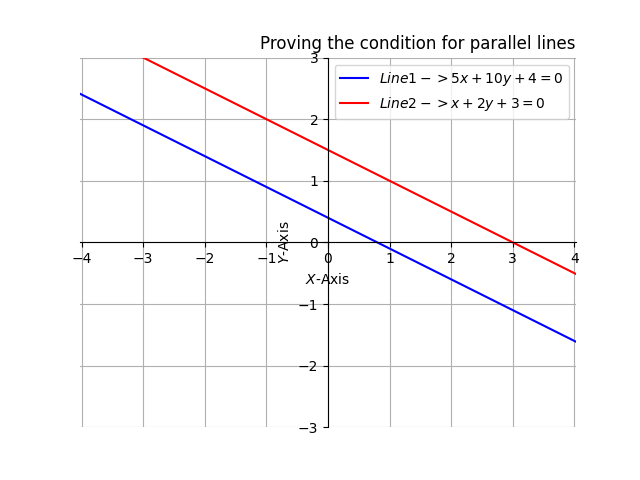
\includegraphics[width=0.7\linewidth]{figs/fig1.png}
		\caption{Assuming two lines which satisfy the above proven condition and proving them with plot. }
	\end{figure}	
\end{document}  







